\documentclass[a4paper,11pt]{article}

\usepackage[spanish]{babel}
\usepackage[utf8]{inputenc}
\usepackage[T1]{fontenc}
\usepackage{graphicx}
\usepackage{float}
\usepackage{hyperref}
\usepackage{listings}
\usepackage{geometry}
\usepackage{amsmath}
\usepackage{subcaption}
\usepackage{float}

\geometry{margin=2.5cm}


\hypersetup{
	colorlinks=true,
	linkcolor=black,
	urlcolor=blue,
	pdfborder={0 0 0}, 
	citecolor=black,
	pdfborderstyle={/S/U/W 1} 
}

\title{Clasificador de Señales en Tiempo Real sobre STM32 utilizando FreeRTOS y NanoEdge AI}
\author{Matías Oliva}
\date{\today}

\begin{document}

\maketitle

\tableofcontents
\newpage

\section{Introducción}

Este informe describe el desarrollo de un sistema embebido capaz de generar, adquirir y clasificar señales en tiempo real utilizando una placa STM32 NUCLEO-U575ZI-Q.

El proyecto combina técnicas de procesamiento digital de señales, sistemas operativos de tiempo real y aprendizaje automático embebido mediante NanoEdge AI Studio.

El objetivo principal es identificar automáticamente diferentes formas de onda generadas por el propio sistema utilizando un modelo de clasificación ejecutado localmente en el microcontrolador.

El proyecto está disponible en \url{https://github.com/ushikawa93/signal_classifier_with_rtos_stm32}.

\section{Objetivos}

\begin{itemize}
\item Generar señales sinusoidales, cuadradas y triangulares utilizando el DAC.
\item Adquirir las señales mediante el ADC.
\item Construir un dataset para entrenamiento.
\item Entrenar un clasificador utilizando NanoEdge AI Studio.
\item Implementar el modelo en un STM32.
\item Utilizar FreeRTOS para coordinar las distintas tareas del sistema.
\item Desarrollar una interfaz gráfica para monitoreo y captura de datos.
\end{itemize}

\section{Hardware Utilizado}

\begin{itemize}
\item STM32 NUCLEO-U575ZI-Q
\item DAC interno
\item ADC interno
\item Comunicación UART
\item Cable de conexión DAC-ADC
\end{itemize}

\begin{figure}[H]
\centering
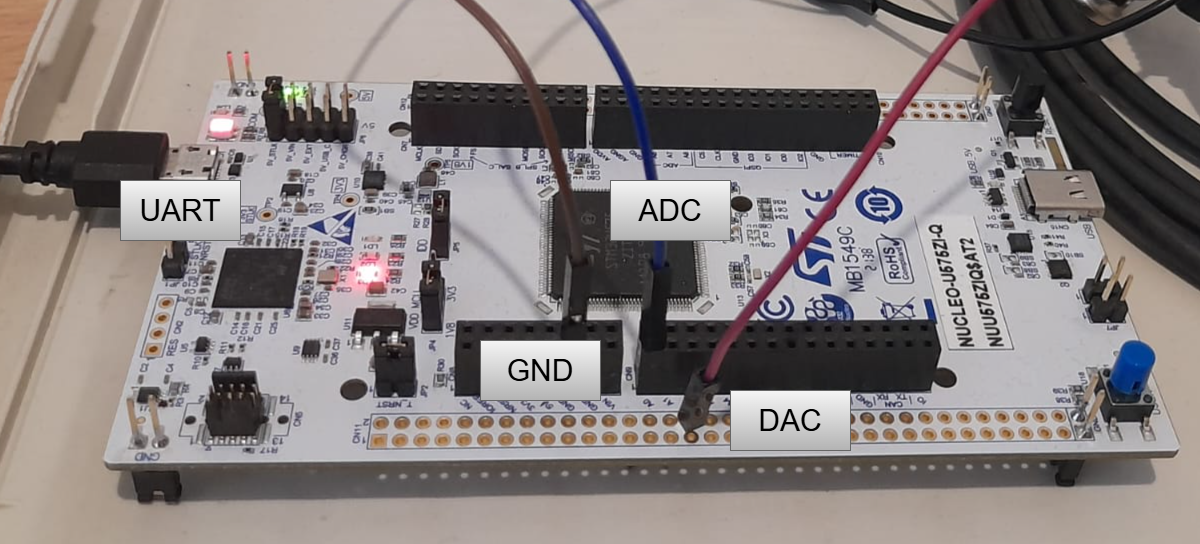
\includegraphics[scale=0.3]{imagenes/FotoHW.png}
\caption{Montaje experimental}
\end{figure}

\section{Arquitectura General}

La arquitectura implementada se basa en la generación de señales mediante DAC, adquisición mediante ADC y posterior clasificación utilizando un modelo de Machine Learning.

\begin{figure}[H]
\centering
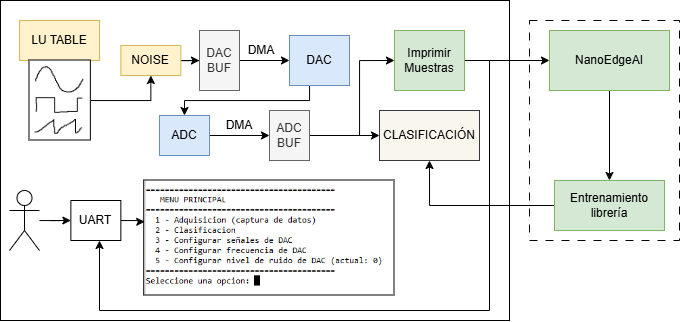
\includegraphics[scale=0.6]{imagenes/EsquemaGeneral.png}
\caption{Arquitectura general}
\end{figure}

\section{Interface de usuario (tarea \texttt{StartUartTask})}

A través del puerto UART el sistema presenta al usuario un menú definido en el header \texttt{menu.h}. En este se le presentan las opciones:

\begin{itemize}
	\item 1 - Adquisicion (captura de datos)
	\item 2 - Clasificacion
	\item 3 - Configurar señales de DAC
	\item 4 - Configurar frecuencia de DAC
	\item 5 - Configurar nivel de ruido de DAC
\end{itemize}

La operación del menú y su derivación a las tareas correspondientes están controladas por la tarea \texttt{StartUartTask}.

\section{Generación de Señales (tarea \texttt{StartDacTask})}

La generación de señales se implementó utilizando:

\begin{itemize}
\item DAC interno (12 bits).
\item DMA en modo circular.
\item Temporizador como trigger.
\item Tablas precalculadas de muestras.
\item Generador de ruido interno del STM32.
\end{itemize}

Las formas de onda implementadas son:

\begin{itemize}
\item Sinusoidal.
\item Cuadrada.
\item Triangular.
\end{itemize}


\subsection{Control del DAC}

La tarea \texttt{StartDacTask} (definido en \texttt{app\_freertos.h}) junto con el header \texttt{signals.h} controlan la operación del DAC.

Esta tarea comienza agregándole ruido a las LU tables (\texttt{generateSignalsWithNoise(int)}) y luego lanza el DAC por DMA. Este esquema tiene la limitación de que el ruido se calcula solo en este punto, por lo que todos los ciclos de la señal tienen los mismos esquemas de ruido (es decir, el ruido es periódico). En un futuro podría mejorarse este punto recalculando las tablas en alguna interrupción que se de al finalizar el buffer del DMA. 

La transferencia memoria- DAC es disparada por el temporizador TIM2. POr defecto este timer esta configurado para generar una señal de 1 segundo de periodo, a partir de una LU table de 128 puntos (triggers cada 1/128 s). 

Esta tarea esta atenta a tres eventos que pueden disparase desde la UART que permiten mnodificar la forma de onda:

\begin{itemize}
	\item \texttt{DAC\_WAVE}: Cambio de la forma de onda.
	\item \texttt{DAC\_NOISE}: Cambia en nivel de ruido en la señal. Para ello detiene el DAC y vuelve a llamar a \texttt{generateSignalsWithNoise(int)}. El nivel de ruido se puede configurar de 0 a 4095 (cuentas del DAC).
	\item \texttt{DAC\_FREQ}: Cambia la frecuencia de actualización del DAC, llamando a la función \texttt{getTIMER\_ DAC(int)} para calcular el periodo del timer deseado a partir de la frecuencia de señal objetivo.
\end{itemize}


\section{Adquisición de Datos (tarea \texttt{StartAdcTask})}

La adquisición se realiza mediante el ADC utilizando DMA circular. Su ejecución esta definida en la tarea \texttt{StartAdcTask}. Esta configura la adquisición por DMA al principio de la operación y luego queda esperando eventos que señalizan bloques de datos listos para procesar.

Para ello se implementó un buffer doble de 256 muestras para permitir el procesamiento simultáneo de los datos mientras continúa la adquisición. La transacción del DMA es disparada por el TIM15, configurado para funcionar a 100 Hz (frecuencia de muestreo).

\begin{figure}[H]
\centering
\includegraphics[scale=0.5]{imagenes/adquisicion_bloques.png}
\caption{Configuración ADC-DMA}
\end{figure}

\subsection{Half Transfer y Transfer Complete}

A medida que se llena el buffer del ADC se disparan dos interrupciones que le avisan a la tarea \texttt{StartAdcTask} que hay datos disponibles para procesar

\begin{itemize}
\item \textbf{Half Complete}. Las primeras 128 muestras del buffer están disponibles
\item \textbf{Complete}. Las segundas 128 muestras del buffer están disponibles.
\end{itemize}

En esta etapa del desarrollo de este proyecto el procesamiento de los datos consiste en imprimir, si el usuario pidió datos desde la UART, los bloques correspondientes a través del puerto serie.


\section{Dataset para Entrenamiento}

Para entrenar el clasificador se implementó un modo de captura que transmite muestras por UART en formato JSON. 

Ejemplo:

\begin{lstlisting}
{
"ts":"00:00:00",
"Muestras":[...]
}
\end{lstlisting}

Cuando el usuario lo pide se imprimen por puerto UART muestras en este formato. Estos se pueden almacenar y utilizar para entrenar algoritmos de clasificación utilizando NanoEdge AI Studio.

\begin{figure}[H]
\centering
\includegraphics[scale=0.8]{imagenes/adquisicion.png}
\caption{Captura de datos para entrenamiento}
\end{figure}

\section{Entrenamiento con NanoEdge AI Studio}

Utilizando la plataforma se adquirieron señales de distintas frecuencias, sinusoidales, 
ondas cuadradas y triangulares que fueron utilizadas para entrenar un modelo de 
clasificación en NanoEdge AI Studio. Para adaptar las señales al formato csv requerido 
por el software se utilizaron scripts disponibles en la carpeta \texttt{/utils} del 
proyecto. En esta carpeta también hay disponible un script de matlab para graficar 
segmentos de las señales obtenidas y verificar su integridad.

\begin{itemize}
	\item \textbf{Dataset utilizado:} Los datos específicos que se utilizaron para 
	entrenar el modelo se encuentran en la carpeta \texttt{nanoEdgeAI/dat}.
	
	\item \textbf{Número de clases:} El modelo se configuró con tres clases: 
	\textit{OndaSinusoidal}, \textit{OndaCuadrada} y \textit{OndaTriangular}.
	
	\item \textbf{Configuración del entrenamiento:} Se empleó la versión 5.1.1 de 
	NanoEdge AI Studio sobre la plataforma NUCLEO-U575ZI-Q, con señales de 128 
	columnas por muestra y 9 señales en total por clase. La búsqueda de la librería 
	óptima se realizó mediante el benchmark automático (\textit{autoML}) de la 
	herramienta, evaluando 17838 librerías candidatas durante 42 minutos con la 
	configuración por defecto.
	
	\item \textbf{Resultados obtenidos:} El benchmark finalizó seleccionando una 
	librería con un \textit{Quality Index} de 99/100 puntos y una 
	\textit{Balanced Accuracy} del 100\%, con un consumo de memoria de 2.4 KB de 
	RAM (incluyendo buffer de 0.6 KB) y 2.7 KB de Flash. La matriz de confusión 
	sobre el conjunto de validación no presentó ningún error de clasificación entre 
	las tres clases, tal como se muestra en la Figura~\ref{fig:nanoedge_resultado}.
\end{itemize}

\begin{figure}[H]
	\centering
	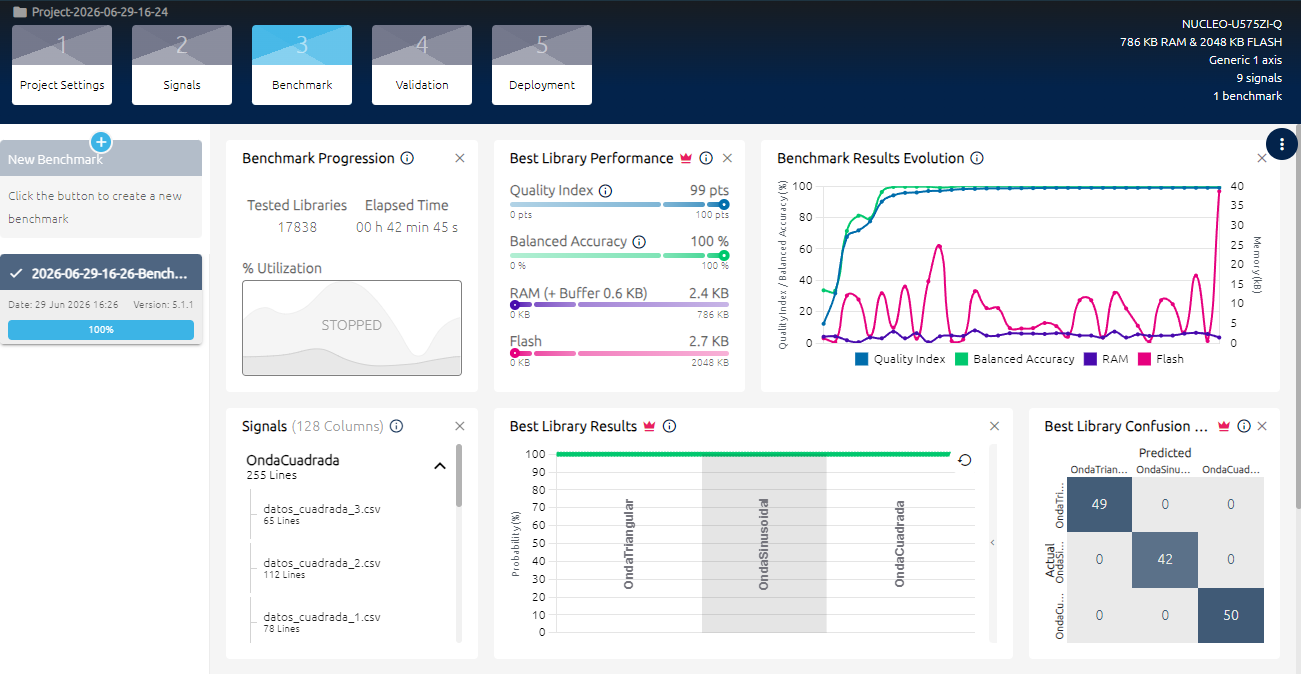
\includegraphics[width=0.9\textwidth]{imagenes/nanoEdgeAI.png}
	\caption{Resultados finales del benchmark en NanoEdge AI Studio.}
	\label{fig:nanoedge_resultado}
\end{figure}


\section{Implementación del Modelo en STM32}

El modelo generado fue integrado al firmware mediante las bibliotecas proporcionadas por NanoEdge AI Studio.

El modelo se inicializa antes de lanzar las tareas, mediante la funcion \texttt{neai\_classification\_init()} provista en la librería.

Luego, dentro de la tarea que controla el UART en la librería, se agregó la clasificación de señales. En este punto, cuando es requerido por el usuario se utiliza la función \texttt{neai\_classification()}, pasandole el contenido del buffer proveniente del ADC que este completo en ese momento (puede ser la primera o la segunda mitad del ADC\_BUF). Antes de utilizarse directamente las muestras se conviertes de entero a punto flotante, por requerimientos de la librería.

Usando este esquema el sistema decide entre alguna de las tres ondas lo que esta muestreando en el ADC, y expone los resultados junto con el nivel de similaridad obtenido.

\begin{figure}[H]
	\centering
	\fbox{\parbox{0.8\textwidth}{\centering
			Captura de pantalla de clasificador}}
	\caption{Proceso de clasificación}
\end{figure}

\section{Migración a FreeRTOS}

Inicialmente el sistema fue desarrollado utilizando una arquitectura secuencial, con modods configurados a través de \texttt{defines}. Esta implementación preeliminar está disponible en \url{https://github.com/ushikawa93/signal_classifier_stm32}.

Posteriormente se migró a FreeRTOS para mejorar la organización del software y desacoplar las distintas funcionalidades.





\section{Aplicación de Monitoreo en Python}

Se desarrolló una aplicación de escritorio utilizando PySide6 para interactuar con el sistema.

Las funcionalidades implementadas incluyen:

\begin{itemize}
\item Conexión serie.
\item Visualización de mensajes UART.
\item Captura de buffers.
\item Graficación en tiempo real.
\item Exportación de logs.
\end{itemize}

Esta implementación está disponible en \texttt{/python\_gui}, con un ejecutable ubicado en \texttt{/python\_ gui/dist/main.exe}

\begin{figure}[H]
	\centering
	\begin{subfigure}[b]{0.48\textwidth}
		\centering
		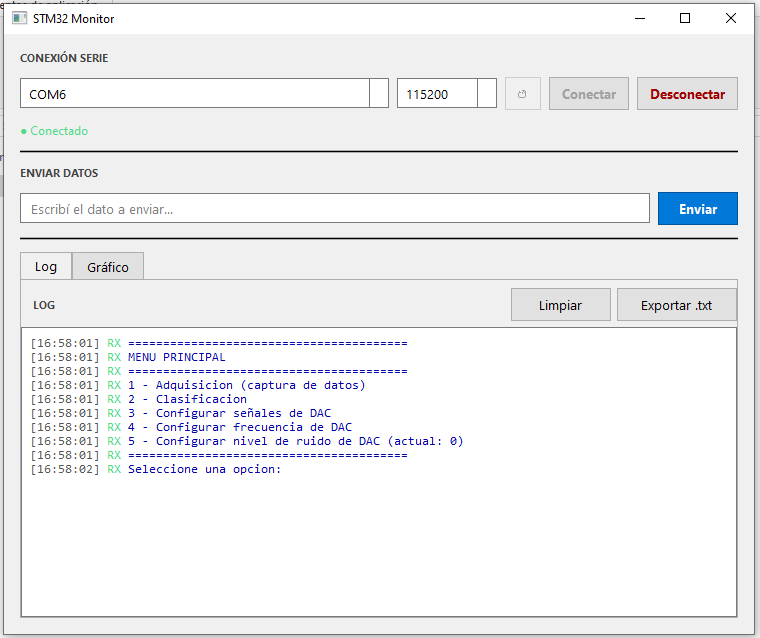
\includegraphics[width=\textwidth]{imagenes/python_gui_1.png}
		\caption{Descripción imagen 1}
		\label{fig:img1}
	\end{subfigure}
	\hfill
	\begin{subfigure}[b]{0.48\textwidth}
		\centering
		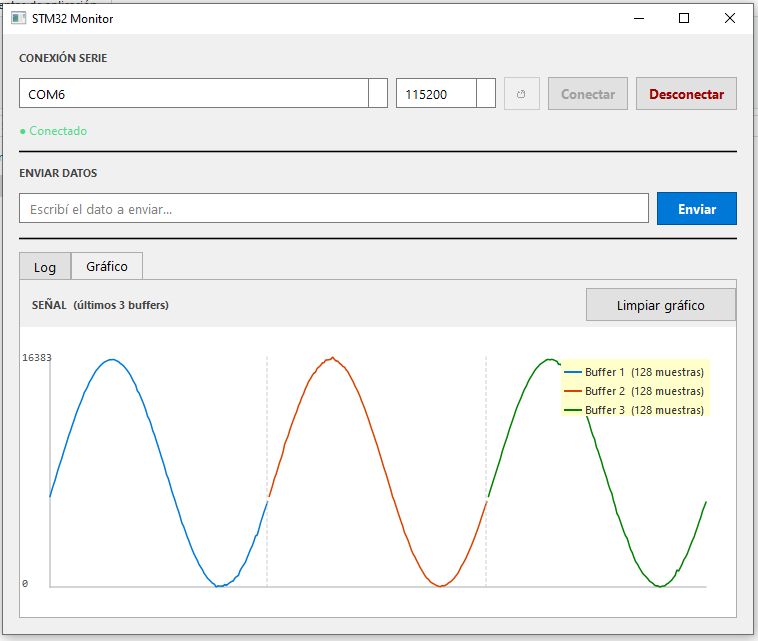
\includegraphics[width=\textwidth]{imagenes/python_gui_2.png}
		\caption{Descripción imagen 2}
		\label{fig:img2}
	\end{subfigure}
	\caption{Aplicación de Monitoreo en Python}
	\label{fig:monitoreo_python}
\end{figure}



\section{Resultados}

Presentar ejemplos de:

\begin{itemize}
\item Señales adquiridas.
\item Clasificaciones obtenidas.
\item Nivel de confianza.
\item Desempeño del sistema.
\end{itemize}

\begin{figure}[H]
\centering
\fbox{\parbox{0.8\textwidth}{\centering
Insertar resultados de clasificación}}
\caption{Resultados obtenidos}
\end{figure}

\section{Conclusiones}

El proyecto permitió integrar distintas tecnologías dentro de una única plataforma embebida:

\begin{itemize}
\item STM32.
\item DMA.
\item FreeRTOS.
\item NanoEdge AI.
\item Comunicación UART.
\item Aplicaciones de escritorio en Python.
\end{itemize}

Además, se obtuvo un sistema capaz de clasificar señales en tiempo real utilizando recursos limitados de procesamiento.

\section{Trabajo Futuro}

\begin{itemize}
\item Incorporar señales externas.
\item Agregar nuevas clases.
\item Implementar FFT en tiempo real.
\item Incorporar almacenamiento en memoria SD.
\item Visualización remota mediante red.
\end{itemize}

\end{document}
